%%%%%%%%%%%%%%%%%%%%%%%%%%%%%%%%%%%%%%
%%%%%%%%%%%%%%%%%%%%%%%%%%%%%%%%%%%%%%
% Do not edit the TeX file your work
% will be overwritten.  Edit the RnW
% file instead.
%%%%%%%%%%%%%%%%%%%%%%%%%%%%%%%%%%%%%%
%%%%%%%%%%%%%%%%%%%%%%%%%%%%%%%%%%%%%%




\newcommand{\FunctionPathsMultFig}{

%<<mult_path, cache=cache, fig.show='hold', fig.cap=fig_cap>>=
\begin{knitrout}
\definecolor{shadecolor}{rgb}{0.969, 0.969, 0.969}\color{fgcolor}

{\centering 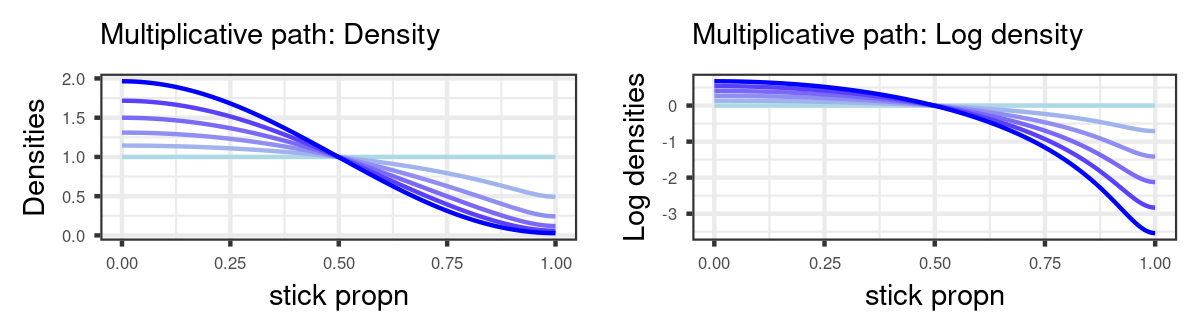
\includegraphics[width=0.980\linewidth,height=0.274\linewidth]{figure/mult_path-1} 

}



\end{knitrout}
}


\newcommand{\FunctionPathsLinFig}{

%<<lin_path, cache=cache, fig.show='hold', fig.cap=fig_cap>>=
\begin{knitrout}
\definecolor{shadecolor}{rgb}{0.969, 0.969, 0.969}\color{fgcolor}

{\centering 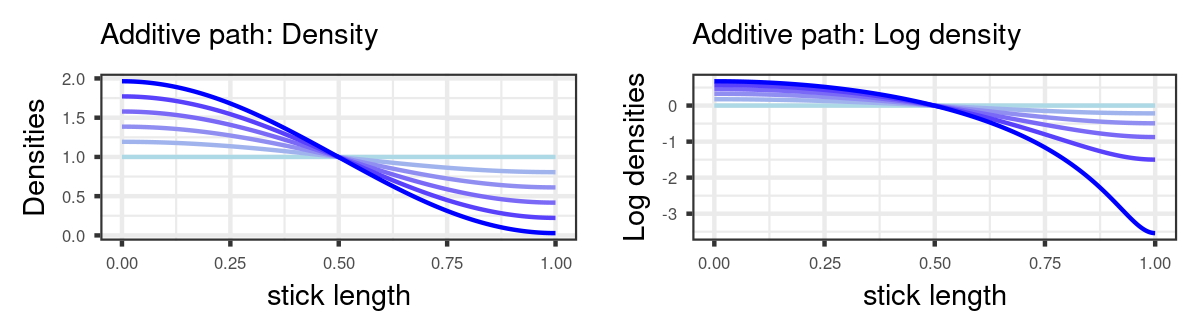
\includegraphics[width=0.980\linewidth,height=0.274\linewidth]{figure/lin_path-1} 

}



\end{knitrout}
}


\newcommand{\FunctionBallFig}{

\begin{knitrout}
\definecolor{shadecolor}{rgb}{0.969, 0.969, 0.969}\color{fgcolor}\begin{figure}[!h]

{\centering 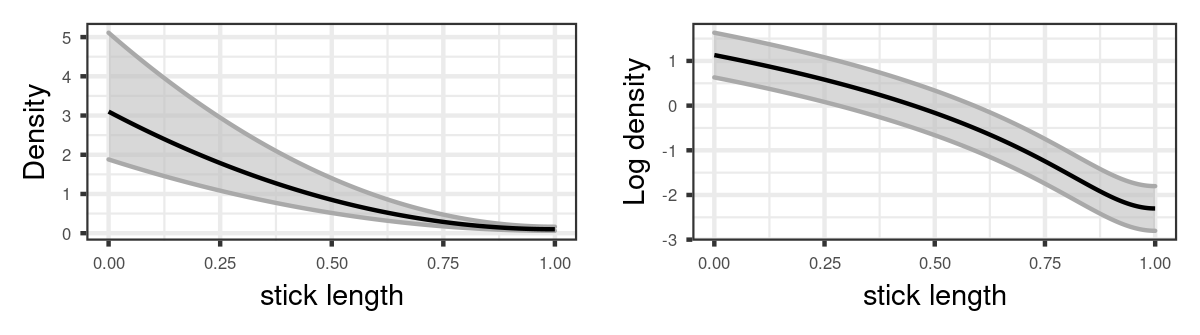
\includegraphics[width=0.980\linewidth,height=0.274\linewidth]{figure/func_ball-1} 

}

\caption[An $\linf{\cdot}$ ball]{An $\linf{\cdot}$ ball.}\label{fig:func_ball}
\end{figure}


\end{knitrout}
}




\newcommand{\FunctionDistFig}{

\begin{knitrout}
\definecolor{shadecolor}{rgb}{0.969, 0.969, 0.969}\color{fgcolor}

{\centering 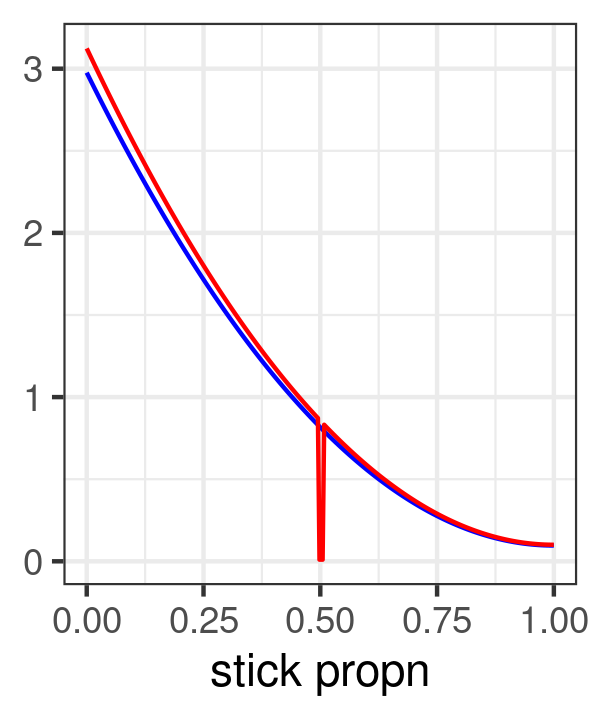
\includegraphics[width=0.490\linewidth,height=0.588\linewidth]{figure/func_dist-1} 

}



\end{knitrout}
}
